%% abtex2-modelo-artigo.tex, v-1.9.6 laurocesar
%% Copyright 2012-2016 by abnTeX2 group at http://www.abntex.net.br/ 
%%
%% This work may be distributed and/or modified under the
%% conditions of the LaTeX Project Public License, either version 1.3
%% of this license or (at your option) any later version.
%% The latest version of this license is in
%%   http://www.latex-project.org/lppl.txt
%% and version 1.3 or later is part of all distributions of LaTeX
%% version 2005/12/01 or later.
%%
%% This work has the LPPL maintenance status `maintained'.
%% 
%% The Current Maintainer of this work is the abnTeX2 team, led
%% by Lauro César Araujo. Further information are available on 
%% http://www.abntex.net.br/
%%
%% This work consists of the files abntex2-modelo-artigo.tex and
%% abntex2-modelo-references.bib
%%

% ------------------------------------------------------------------------
% ------------------------------------------------------------------------
% abnTeX2: Modelo de Artigo Acadêmico em conformidade com
% ABNT NBR 6022:2003: Informação e documentação - Artigo em publicação 
% periódica científica impressa - Apresentação
% ------------------------------------------------------------------------
% ------------------------------------------------------------------------

\documentclass[
    % -- opções da classe memoir --
    article,            % indica que é um artigo acadêmico
    11pt,               % tamanho da fonte
    oneside,            % para impressão apenas no recto. Oposto a twoside
    a4paper,            % tamanho do papel. 
    % -- opções da classe abntex2 --
    %chapter=TITLE,     % títulos de capítulos convertidos em letras maiúsculas
    %section=TITLE,     % títulos de seções convertidos em letras maiúsculas
    %subsection=TITLE,  % títulos de subseções convertidos em letras maiúsculas
    %subsubsection=TITLE % títulos de subsubseções convertidos em letras maiúsculas
    % -- opções do pacote babel --
    english,            % idioma adicional para hifenização
    brazil,             % o último idioma é o principal do documento
    sumario=tradicional,
    ]{abntex2}


% ---
% PACOTES
% ---
\usepackage[table,xcdraw]{xcolor}

% ---
% Pacotes fundamentais 
% ---
\usepackage{lmodern}            % Usa a fonte Latin Modern
\usepackage[T1]{fontenc}        % Selecao de codigos de fonte.
\usepackage[utf8]{inputenc}     % Codificacao do documento (conversão automática dos acentos)
\usepackage{indentfirst}        % Indenta o primeiro parágrafo de cada seção.
\usepackage{nomencl}            % Lista de simbolos
\usepackage{color}              % Controle das cores
\usepackage{graphicx}           % Inclusão de gráficos
\usepackage{microtype}          % para melhorias de justificação
% ---
        
% ---
% Pacotes adicionais, usados apenas no âmbito do Modelo Canônico do abnteX2
% ---
\usepackage{lipsum}             % para geração de dummy text
\usepackage{fancyvrb}
\usepackage{todonotes}
\usepackage{float}
\usepackage[procnames]{listings}
\usepackage{color}
\usepackage{amsmath}
\usepackage{cancel}
% ---
        
% ---
% Pacotes de citações
% ---
\usepackage[brazilian,hyperpageref]{backref}     % Paginas com as citações na bibl
\usepackage[alf]{abntex2cite}   % Citações padrão ABNT
% ---

% ---
% Configurações do pacote backref
% Usado sem a opção hyperpageref de backref
\renewcommand{\backrefpagesname}{Citado na(s) página(s):~}
% Texto padrão antes do número das páginas
\renewcommand{\backref}{}
% Define os textos da citação
\renewcommand*{\backrefalt}[4]{
    \ifcase #1 %
        Nenhuma citação no texto.%
    \or
        Citado na página #2.%
    \else
        Citado #1 vezes nas páginas #2.%
    \fi}%
% ---

% ---
% Informações de dados para CAPA e FOLHA DE ROSTO
% ---
\titulo{Exercício INE5644 - Data Mining\\ 
        Classificação - Árvores de Decisão}
\autor{Bruno Marques do Nascimento\thanks{brunomn95@gmail.com \hspace{1mm} - \hspace{1mm} Universidade Federal de Santa Catarina \hspace{1mm} - \hspace{1mm} Matrícula: 15104098}}
\instituicao{Universidade Federal de Santa Catarina}
\local{Florianópolis - SC, Brasil}
\data{23 de Abril de 2018}
% ---

% ---
% Configurações de aparência do PDF final

% alterando o aspecto da cor azul
\definecolor{blue}{RGB}{41,5,195}

% informações do PDF
\makeatletter
\hypersetup{
        %pagebackref=true,
        pdftitle={\@title}, 
        pdfauthor={\@author},
        pdfsubject={Modelo de artigo científico com abnTeX2},
        pdfcreator={LaTeX with abnTeX2},
        pdfkeywords={abnt}{latex}{abntex}{abntex2}{atigo científico}, 
        colorlinks=true,            % false: boxed links; true: colored links
        linkcolor=blue,             % color of internal links
        citecolor=blue,             % color of links to bibliography
        filecolor=magenta,              % color of file links
        urlcolor=blue,
        bookmarksdepth=4
}
\makeatother
% --- 

% ---
% compila o indice
% ---
\makeindex
% ---

% ---
% Altera as margens padrões
% ---
\setlrmarginsandblock{3cm}{3cm}{*}
\setulmarginsandblock{3cm}{3cm}{*}
\checkandfixthelayout
% ---

% --- 
% Espaçamentos entre linhas e parágrafos 
% --- 

% O tamanho do parágrafo é dado por:
\setlength{\parindent}{1.3cm}

% Controle do espaçamento entre um parágrafo e outro:
\setlength{\parskip}{0.2cm}  % tente também \onelineskip

% Espaçamento simples
\SingleSpacing

% ----
% Início do documento
% ----
\begin{document}

% Seleciona o idioma do documento (conforme pacotes do babel)
%\selectlanguage{english}
\selectlanguage{brazil}

% Retira espaço extra obsoleto entre as frases.
\frenchspacing 

% ----------------------------------------------------------
% ELEMENTOS PRÉ-TEXTUAIS
% ----------------------------------------------------------

%---
%
% Se desejar escrever o artigo em duas colunas, descomente a linha abaixo
% e a linha com o texto ``FIM DE ARTIGO EM DUAS COLUNAS''.
% \twocolumn[           % INICIO DE ARTIGO EM DUAS COLUNAS
%
%---
% página de titulo

\maketitle


% ----------------------------------------------------------
% ELEMENTOS TEXTUAIS
% ----------------------------------------------------------
\textual

% ----------------------------------------------------------
% Introdução
% ----------------------------------------------------------
% \section*{Introdução}
% \addcontentsline{toc}{section}{Introdução}

\section*{\textbf{Contexto:}}
\addcontentsline{toc}{section}{Contexto}

Considere o seguinte conjunto de treinamento, em que cada exemplo é definido por três atributos (A,B,C) e a classe X.

\begin{table}[H]
\centering
\caption{Conjunto de treinamento}
\label{train_table}
\begin{tabular}{|c|c|c|c|c|}
\hline
\rowcolor[HTML]{34CDF9} 
            & \textbf{A} & \textbf{B} & \textbf{C} & \textbf{X} \\ \hline
\textbf{X1} & 1          & 1          & 3          & P          \\ \hline
\textbf{X2} & 1          & 2          & 4          & P          \\ \hline
\textbf{X3} & 2          & 2          & 4          & N          \\ \hline
\textbf{X4} & 2          & 1          & 4          & N          \\ \hline
\end{tabular}
\end{table}

Sabendo que:
\begin{itemize}
    \item$\boldsymbol{Entropia(S) = - (p_+ \log_2 p_+) - (p_- \log_2 p_-)}$
    \item$\boldsymbol{Ganho(S, A) = Entropia(S) - \sum ((|Sv| / |S|) * Entropia (Sv))}$, onde:
    \begin{itemize}
        \item\textbf{Ganho(S, A)}: ganho do atributo A sobre o conjunto S
        \item\textbf{Sv}: subconjunto de S para um valor do atributo A.
        \item\textbf{|Sv|}: número de elementos de Sv.
        \item\textbf{|S|}: número de elementos de S.
    \end{itemize}
\end{itemize}

\begin{table}[H]
\centering
\caption{Dados fornecidos}
\label{logs_table}
\begin{tabular}{|l c r|}
\hline
\rowcolor[HTML]{34CDF9} 
$\log_21$     & = & $0$      \\ \hline
$\log_20.5$   & = & $-1$     \\ \hline
\rowcolor[HTML]{34CDF9} 
$\log_20.25$  & = & $-2$     \\ \hline
$\log_20.75$  & = & $-0.415$ \\ \hline
\rowcolor[HTML]{34CDF9} 
$\log_20.333$ & = & $-1.585$ \\ \hline
$\log_20.667$ & = & $-0.585$ \\ \hline
\end{tabular}
\end{table}


\section*{\textbf{Perguntas:}}
% ----------------------------------------------------------
% a)
% ----------------------------------------------------------
\subsection*{\textbf{a) Qual a incerteza (entropia) associada ao conjunto de treinamento inicial?}}
\addcontentsline{toc}{subsection}{a)}

\begin{align*}
Entropia(S) &= - (\tfrac{2}{4} \times \log_2 \tfrac{2}{4}) - (\tfrac{2}{4} \times \log_2 \tfrac{2}{4})   \\ 
            &= - (0.5 \times \log_2 0.5) - (0.5 \times \log_2 0.5)                                       \\
            &= - (0.5 \times -1) - (0.5 \times -1)                                                       \\
            &= - (-0.5) - (-0.5)                                                                         \\
            &= 0.5 + 0.5                                                                                 \\
            &= 1                                                                                       \\\\
Entropia(A=1) &= - (\tfrac{2}{2} \times \log_2 \tfrac{2}{2}) - (\tfrac{0}{2} \times \log_2 \tfrac{0}{2}) \\ 
              &= - (1 \times \log_2 1) - \cancel{(0 \times \log_2 \tfrac{0}{2})}                         \\
              &= - (1 \times 0)                                                                          \\
              &= 0                                                                                     \\\\
Entropia(A=2) &= - (\tfrac{0}{2} \times \log_2 \tfrac{0}{2}) - (\tfrac{2}{2} \times \log_2 \tfrac{2}{2}) \\ 
              &= - \cancel{(0 \times \log_2 \tfrac{0}{2})} - (1 \times \log_2 1)                         \\
              &= - (1 \times 0)                                                                          \\
              &= 0                                                                                     \\\\
Entropia(B=1) &= - (\tfrac{1}{2} \times \log_2 \tfrac{1}{2}) - (\tfrac{1}{2} \times \log_2 \tfrac{1}{2}) \\ 
              &= - (0.5 \times \log_2 0.5) - (0.5 \times \log_2 0.5)                                     \\
              &= - (0.5 \times -1) - (0.5 \times -1)                                                     \\
              &= 1                                                                                     \\\\
Entropia(B=2) &= - (\tfrac{1}{2} \times \log_2 \tfrac{1}{2}) - (\tfrac{1}{2} \times \log_2 \tfrac{1}{2}) \\ 
              &= - (0.5 \times \log_2 0.5) - (0.5 \times \log_2 0.5)                                     \\
              &= - (0.5 \times -1) - (0.5 \times -1)                                                     \\
              &= 1                                                                                     \\\\
Entropia(C=3) &= - (\tfrac{1}{1} \times \log_2 \tfrac{1}{1}) - (\tfrac{0}{1} \times \log_2 \tfrac{0}{1}) \\ 
              &= - (1 \times \log_2 1) - \cancel{(0 \times \log_2 \tfrac{0}{1})}                         \\
              &= - (1 \times 0)                                                                          \\
              &= 0                                                                                     \\\\
Entropia(C=4) &= - (\tfrac{1}{3} \times \log_2 \tfrac{1}{3}) - (\tfrac{2}{3} \times \log_2 \tfrac{2}{3}) \\ 
              &= - (0.333 \times \log_2 0.333) - (0.667 \times \log_2 0.667)                             \\
              &= - (0.333 \times -1.585) - (0.667 \times -0.585)                                         \\
              &= 0.918                                                                                 \\\\
\end{align*}

% ----------------------------------------------------------
% a)
% ----------------------------------------------------------
\subsection*{\textbf{b) Qual o Ganho de Informação para cada um dos atributos?}}
\addcontentsline{toc}{subsection}{b)}

\begin{align*}
Ganho(S, A) &= 1 - ((\tfrac{2}{4}) \times 0) - ((\tfrac{2}{4}) \times 0)      \\ 
            &= 1                                                            \\\\
Ganho(S, B) &= 1 - ((\tfrac{2}{4}) \times 1) - ((\tfrac{2}{4}) \times 1)      \\ 
            &= 0                                                            \\\\
Ganho(S, C) &= 1 - ((\tfrac{1}{4}) \times 0) - ((\tfrac{3}{4}) \times 0.918)  \\ 
            &= 0.3115
\end{align*}

% ----------------------------------------------------------
% a)
% ----------------------------------------------------------
\subsection*{\textbf{c) Face a este resultado, qual seria a árvore de decisão obtida para este conjunto de treinamento, construída de acordo com o critério de maximização do ganho de informação?}}
\addcontentsline{toc}{subsection}{c)}

\begin{figure}[H]
    \label{decision_tree_fig}
    \caption{Árvore de decisão}
    \begin{center}
        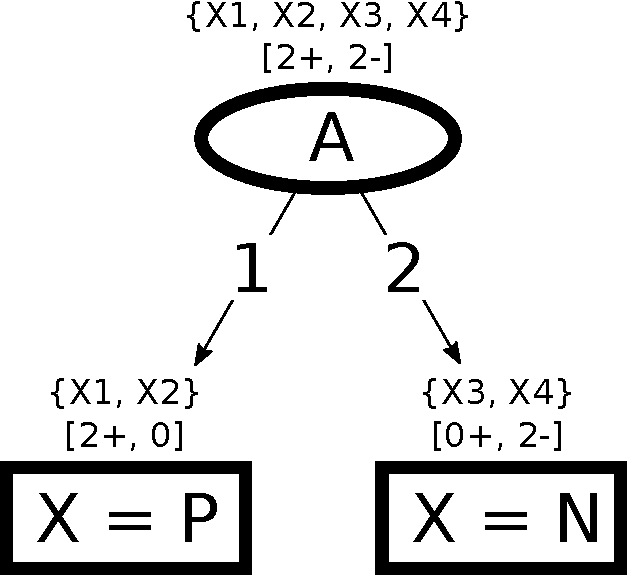
\includegraphics[scale=0.5]{imgs/decision-tree.pdf}
    \end{center}
    % \legend{Fonte: \citeonline[p. 24]{araujo2012}}
\end{figure}

% ---
% Finaliza a parte no bookmark do PDF, para que se inicie o bookmark na raiz
% ---
\bookmarksetup{startatroot}% 
% ---

% ---
% Conclusão
% ---
% \section*{Considerações finais}
% \addcontentsline{toc}{section}{Considerações finais}

% ----------------------------------------------------------
% ELEMENTOS PÓS-TEXTUAIS
% ----------------------------------------------------------
\postextual

% ----------------------------------------------------------
% Referências bibliográficas
% ----------------------------------------------------------
\nocite{slides_aula}
\bibliography{bibliography}

\end{document}
